\documentclass[english,11pt]{beamer}

\DeclareMathOperator{\Cov}{Cov}
\DeclareMathOperator{\Var}{Var}
\DeclareMathOperator{\E}{\mathbb{E}}
\DeclareMathOperator{\Proba}{\mathbb{P}}

\newcommand{\Covb}[2]{\ensuremath{\Cov\!\left[#1,#2\right]}}
\newcommand{\Eb}[1]{\ensuremath{\E\!\left[#1\right]}}
\newcommand{\Pb}[1]{\ensuremath{\Proba\!\left[#1\right]}}
\newcommand{\Varb}[1]{\ensuremath{\Var\!\left[#1\right]}}

% norm
\newcommand{\norm}[1]{\| #1 \|}

\newcommand{\indep}{\rotatebox[origin=c]{90}{$\models$}}





\usepackage{mathptmx,amsmath,amssymb,graphicx,bibentry,bbm,babel,ragged2e}

\makeatletter

\newcommand{\noun}[1]{\textsc{#1}}
\newcommand{\jitem}[1]{\item \begin{justify} #1 \end{justify} \vfill{}}
\newcommand{\sframe}[2]{\frame{\frametitle{#1} #2}}

\newenvironment{centercolumns}{\begin{columns}[c]}{\end{columns}}
%\newenvironment{jitem}{\begin{justify}\begin{itemize}}{\end{itemize}\end{justify}}

\usetheme{Warsaw}
\setbeamertemplate{footline}[text line]{}
\setbeamertemplate{headline}{}
\setbeamercolor{structure}{fg=purple!50!blue, bg=purple!50!blue}

\setbeamersize{text margin left=15pt,text margin right=15pt}

\setbeamercovered{transparent}


\@ifundefined{showcaptionsetup}{}{%
 \PassOptionsToPackage{caption=false}{subfig}}
\usepackage{subfig}

\usepackage[utf8]{inputenc}
\usepackage[T1]{fontenc}

\usepackage{multirow}

\usepackage{mdframed}


\makeatother


\AtBeginSection[]
{
  \begin{frame}
  \frametitle{Towards geocommons for sustainable territorial planning and management}
  \tableofcontents[currentsection]
  \end{frame}
}

\begin{document}



% Vers des géocommuns pour une gestion durable des territoires
\title{Towards geocommons for sustainable territorial planning and management}

\author{J.~Raimbault$^{1,2,3,4}$\\
\texttt{juste.raimbault@ign.fr}
}


\institute{$^{1}$LASTIG, Univ. Gustave Eiffel, IGN-ENSG\\
$^{2}$CASA, UCL\\
$^{3}$UPS CNRS 3611 ISC-PIF\\
$^{4}$UMR CNRS 8504 G{\'e}ographie-cit{\'e}s
}


\date{\textit{Journ{\'e}es Scientifiques de Rochebrune 2023}\\
31/03/2023
}


\frame{\maketitle}


\section{Digital twins and sustainability}


\sframe{Territorial systems and SDGs}{

%\justify

\textbf{SDG 11}: ``Make cities and human settlements inclusive, safe, resilient, and sustainable'' \cite{nations2015sustainable}

\bigskip

$\rightarrow$ Cities as a transition state? \cite{batty2018inventing} Incubators of social change and innovation, both the source and solution to sustainability issues? \cite{pumain2010theorie}

\bigskip

$\rightarrow$ Environmental Kuznet Curve hypothesis \cite{dinda2004environmental, stern2004rise}: inverted U-shaped relationship between environmental impact and income per-capita; not validated empirically \cite{harbaugh2002reexamining}

\bigskip

$\rightarrow$ Trade-offs between SDGs in \textbf{urban systems} \cite{viguie2012trade}, and more generally \textbf{territorial systems}.


}

\sframe{Research at IGN: Digital twins and sustainability}{

\centering

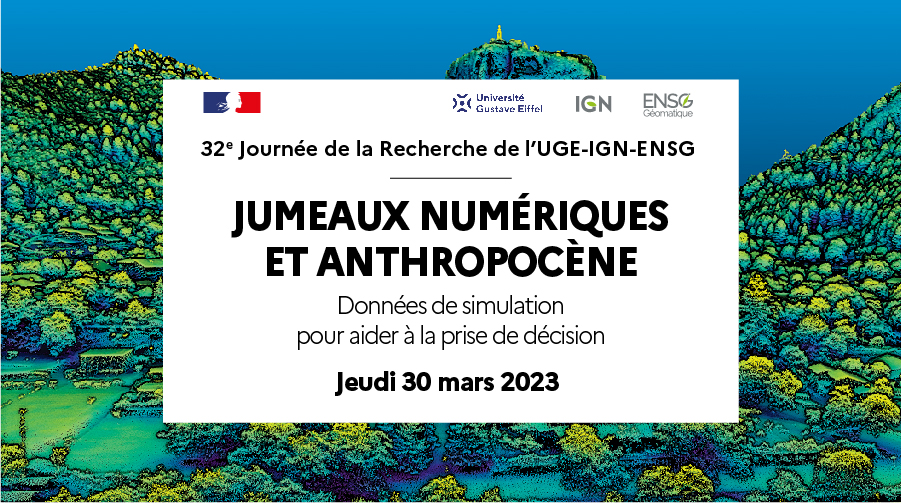
\includegraphics[width=\linewidth]{figures/JR}

}




\sframe{Digital twins and sustainability: literature mapping}{

% si possible carto lit dig twin - sdgs

% Request : "digital twin" AND "sustainable development" (adding "sustainb*" -> too general, include sust economically e.g.)
%   initial corpus?

\justify

\textit{How do the two main themes of the conference go along in the literature?}

\medskip

\textit{What principal fields of study applying digital twins to sustainable development?}


\bigskip
\bigskip

$\rightarrow$ Using the methods and tools of \cite{raimbault2019exploration} \cite{raimbault2021empowering}, we do a systematic literature mapping using citation networks, constructed from google scholar data.

\medskip

$\rightarrow$ Starting from a seed corpus of 100 papers obtained with the request\\
\texttt{"digital twin" AND "sustainable development"}, we retrieve backward citations at depth two, to obtain a corpus of \textbf{14042 papers} with \textbf{24229 citation links}.

\medskip

$\rightarrow$ We analyse the citation network using community detection, to retrieve endogenous research fields.


}

\sframe{Main research areas from the literature mapping}{

\begin{columns}
	\begin{column}{0.6\linewidth}
		\includegraphics[width=1.1\linewidth]{figures/core_zoom}
	\end{column}
	\begin{column}{0.39\linewidth}
		\footnotesize
		\begin{itemize}
		    \item ``Smart manufacturing'' (21.9\%)
			\item Epistemology of DT (14.6\%)
			\item Civil engineering/BIM (11.4\%)
			\item Supply chain (6.8\%)
			\item Circular economy (5.6\%)
			\item Energy systems (5.1\%)
			\item Urban analytics/smart cities (5.0\%)
			\item ``Metaverse'' (4.5\%)
			\item ``Industry 4.0'' (4.2\%)
			\item ``Smart farming'' (4.0\%)
		\end{itemize}
	\end{column}
\end{columns}



}



\sframe{Digital twins: concepts and reality}{

\justify

% dig twins \cite{batty2018digital}

\textbf{Definition of a DT?} Coined in the 2000s from engineering \cite{batty2018digital}

\medskip

{\footnotesize ``\textit{A digital twin is a mirror image of a physical process [\ldots], usually matching exactly the operation of the physical process which takes place in real time.}''}

\medskip

$\rightarrow$ in practice not identical (example for cities: real-time GIS \cite{li2020real}); often not in real time or even dynamical.

\bigskip

The \textbf{link between the model (twin) and the system} is complex: which level of detail, which modelling choices, how to handle the resulting hybrid cyber-physical system? \cite{batty2019map}

``{\footnotesize \textit{A map is not the territory, or is it?}}''
% (inspire houllebeq et Levy) (meaning of representation)

\bigskip

% link with complexity \cite{arcaute2021future}

DT approaches too close to systems engineering, and often miss \textbf{social science/complexity} issues \cite{arcaute2021future}

$\rightarrow$ models at all time scales decision-making in the anthropocene.


}



\sframe{From digital twins to multiple simulation models}{


\justify

\textit{How to link digital twins and decision-making for sustainable development?}

\bigskip
\bigskip

$\rightarrow$ smart cities are on the long run: urban analytics for policy \\
\cite{kandt2021smart}

\bigskip

$\rightarrow$ unpredictability, multi-dimensionality, multi-scalarity of territorial systems: need for multiple models \cite{batty2021multiple}, multiple perspectives\\
 \cite{pumain2020conclusion}

\bigskip

$\rightarrow$ simulation models of territories for sustainable policies\\
\cite{raimbault2020empowering}


}


\section{Geocommons}

\sframe{Digital twins as commons?}{

More general framework of ``\textit{g{\'e}o-communs}'', launched by IGN since January 2021 \url{https://www.ign.fr/institut/la-demarche-geocommuns}.

\smallskip

\begin{center}

\includegraphics[width=0.15\linewidth]{figures/LOGO_IGN.png}

\includegraphics[width=0.54\linewidth]{figures/geocommuns.png}
\end{center}

\smallskip

$\rightarrow$ all IGN data is now open data 

$\rightarrow$ mutualisation, collaboration around tools, methods, databases

$\rightarrow$ public consultation in May 2021 (165 stakeholders from various backgrounds)

\medskip

\footnotesize

\textbf{Definition: } ``\textit{Geographic Information databases co-producted or co-maintained, and co-developped tools and methods, following an open common governance, to garantee a full appropriation by communities of users/producers/stakeholders/citizens}''

}

\sframe{Open questions for geocommons}{

\begin{enumerate}
	\item Governance of geocommons: mediator $\neq$ technical coordinator
	\item Economic model: public service (open public good)
	\item Core data: static digital twin at the national scale?
	\item Data production: e.g. link with OSM
	\item Licence: open licence but not ODbL?
	\item Methods and tools: ecosystem of open source softwares
	\item Open science as a part of geocommons
	\item Crucial role for environmental data
	\item Link with European directives for open data; European geocommons?
\end{enumerate}


}

\sframe{Implementation of geocommons}{

\begin{center}

\includegraphics[width=0.3\linewidth]{figures/fabrique_geocom}\hspace{1cm}

\includegraphics[width=0.3\linewidth]{figures/geoplateforme}
\end{center}

\medskip 

\textit{La Fabrique} as a project incubator, \textit{Geoplateforme} as the future technical basis for data sharing (successor of geoportail)

\medskip

\textbf{Examples of application themes:} public health and environment, renewable energy, urban planning, local governments.

\medskip

% ANCT: agence Nationale de la Cohesion des Territoires ; DINUM: Direction intermin du numerique
\textbf{Examples of current projects:} \textit{Base Adresse Nationale} (ANCT, DINUM, IGN), \textit{Panoramax} (immersive views; OSM, IGN), \textit{BAT-ID} (national building database; CSTB, ADEME, IGN).


}

\sframe{The national Digital Twin and geo-commons}{

\textbf{Current project proposal being prepared at IGN: } a national Digital Twin providing a high resolution 3D model of the country (collaboration IGN, INRIA, CEREMA, still open to other agencies).

\bigskip

\textbf{Main axis:}

\begin{enumerate}
	\item Specification of the 3D model
	\item Production of the 3D model
	\item Updates of the 3D model
	\item Link and integration with other data
	\item Online visualisation and interaction
	\item Simulation: downstream application
\end{enumerate}

\bigskip

% link geocommons, but simu "missed" -> project next proposed as a stronger ocntribution for geocommons towards sust policies

$\rightarrow$ strong interaction with geo-commons expected

$\rightarrow$ however simulation not central (against the strict definition of a DT): \textbf{we propose a project focused on simulation models to contribute to geo-commons}

}



\section{Integrating and validating simulation models}


%%%%
% transition, or intermediate conclusion: sim models at the core of dig twins

% -> for sustainable decision making? -> introduce project

\sframe{Towards sustainable decision making for territories by integrating and validating simulation models}{


\begin{center}
	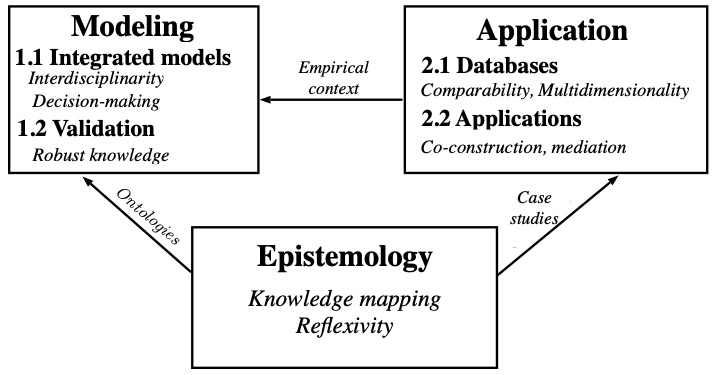
\includegraphics[width=\textwidth]{figures/axes_edited_EN.jpg}	
\end{center}


\textbf{Integrated models} to simulate multiple dimensions of \textbf{urban systems} towards decision-making in the context of \textbf{sustainable transitions}.


}


%   -> need integration and validation of simulation models



\sframe{OpenMOLE: validation of simulation models}{

% https://hackmd.openmole.org/6yuwyo1dR1aulyqy9iZeyQ#PSE-performances

%     Logiciel libre pour l’exploration et l’évaluation de modèles de simulation   Utilisable avec la majorité des modèles de simulation    Propose une méthodologie d’exploration    Délègue le calcul de manière transparente sur cluster et grille
%     150 000 lignes de code ;   16 000 commits  15 versions  60 contributeurs  Des centaines de modèles explorés  Plusieurs milliards d’heures de calcul

\centering

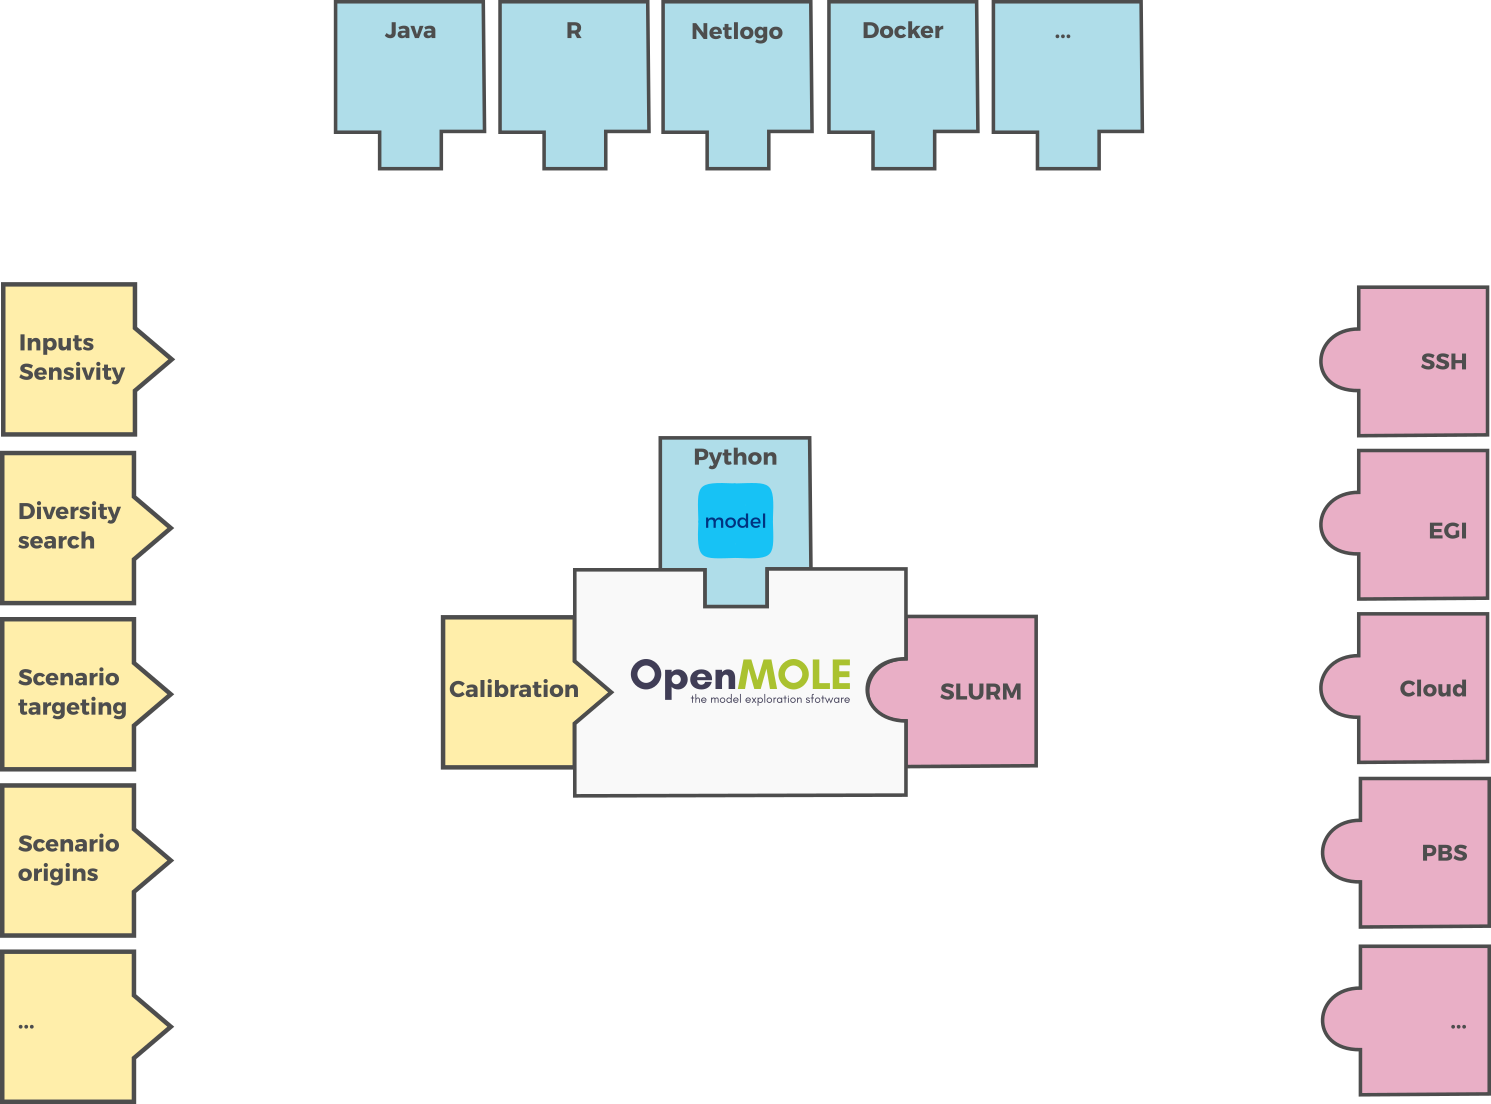
\includegraphics[width=0.85\linewidth]{figures/openmole_axis}

\url{http://openmole.org} \cite{reuillon2013openmole}

}


\sframe{OpenMOLE: objectively the best}{

% + compare dafni!, mention closed solutions oral

\centering

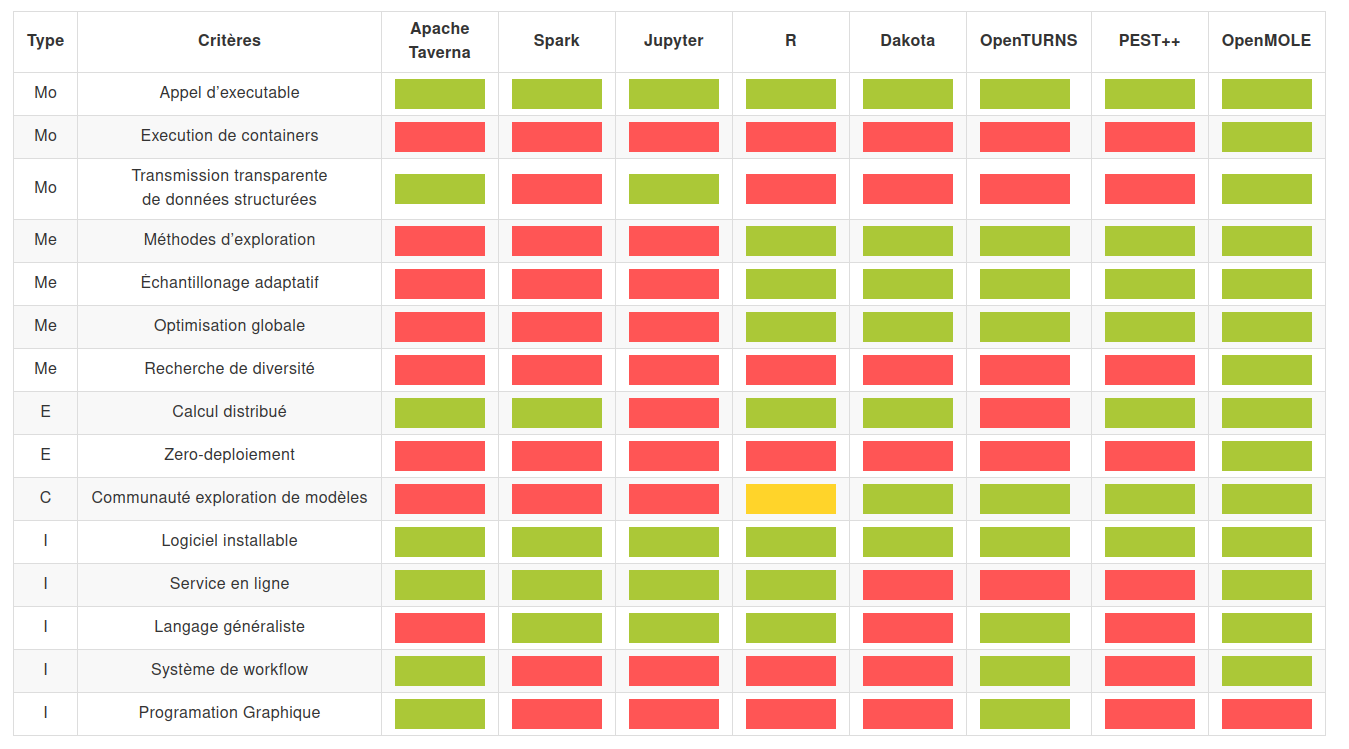
\includegraphics[width=\linewidth]{figures/openmole_benchmark}

}



\sframe{Novel validation methods: spatial sensitivity analysis}{



\centering

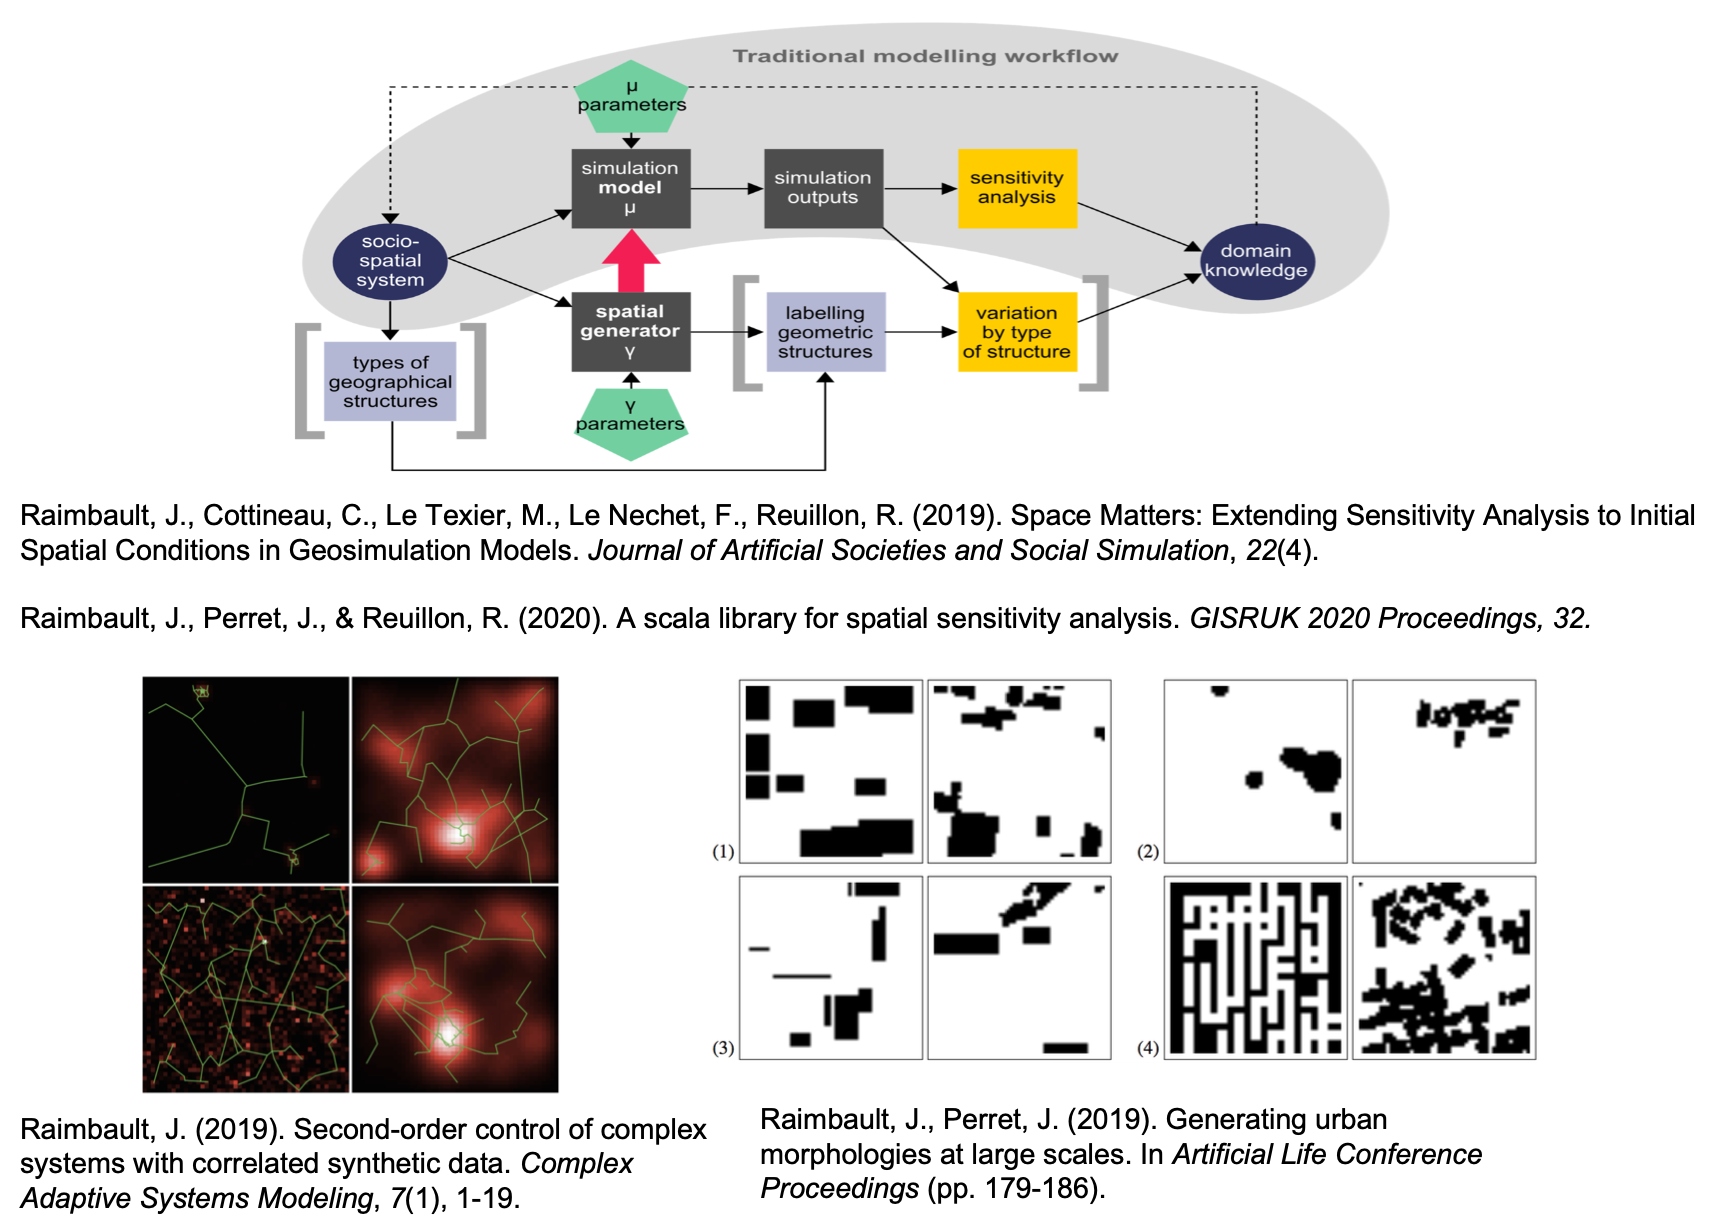
\includegraphics[width=0.95\linewidth]{figures/spatial_sa.png}

\nocite{raimbault2019second}
\nocite{raimbault2019generating}
\nocite{raimbault2019space}

}



\sframe{Model integration: land-use transport interactions}{


\includegraphics[width=0.39\linewidth]{figures/accessp_withbridge_prd_EN.png}
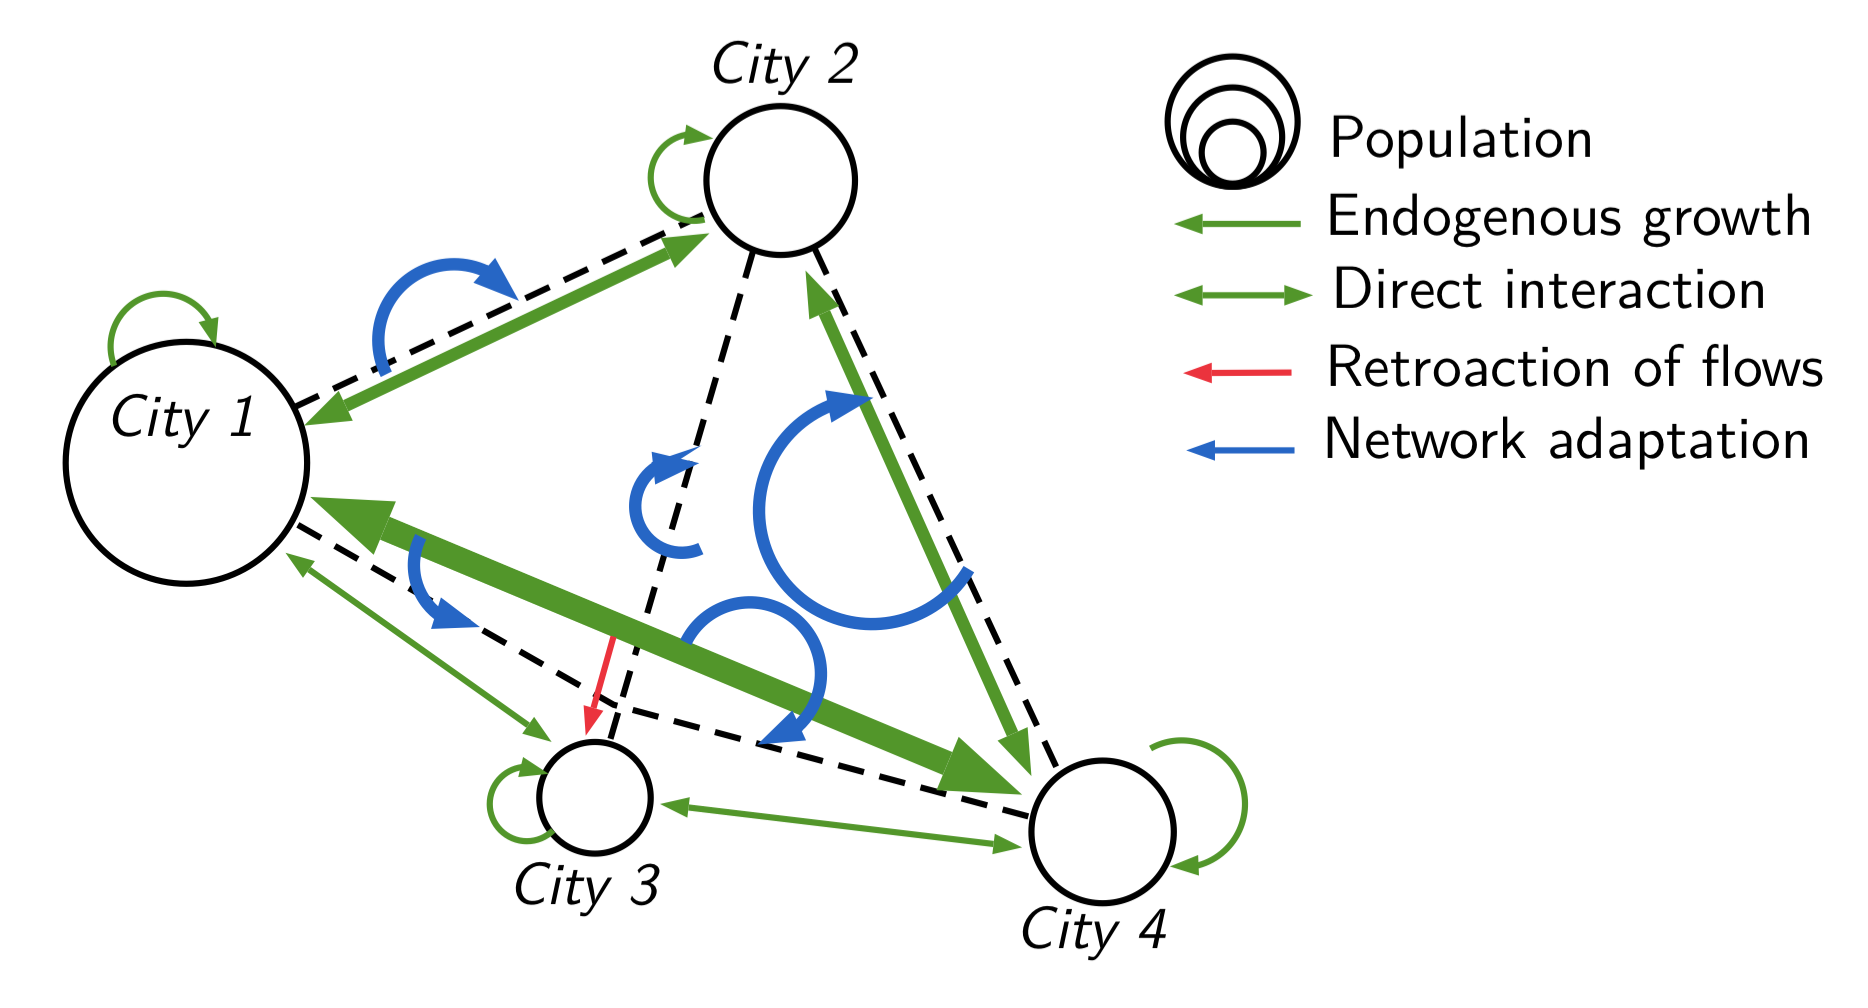
\includegraphics[width=0.6\textwidth]{figures/macrocoevol_en.png}

\medskip


\textit{A modeling approach to the issue of structuring effects of transport infrastructures: co-evolution of networks and territories as a strong model integration}

\bigskip

\tiny
%\textcolor{grey}
Raimbault, J. (2019). Evolving accessibility landscapes: mutations of transportation networks in China. In Aveline-Dubach, N., ed. \textit{Pathways of sustainable urban development across China - the cases of Hangzhou, Datong and Zhuhai}, pp 89-108. Imago. ISBN:978-88-94384-71-0

\nocite{raimbault:halshs-02265423}

\smallskip

Raimbault, J. (2020). Indirect evidence of network effects in a system of cities. Environment and Planning B: Urban Analytics and City Science, 47(1), 138-155.

\nocite{raimbault2020indirect}

\smallskip

Raimbault, J. (2021). Modeling the co-evolution of cities and networks. In Handbook of Cities and Networks. Edward Elgar Publishing.

\nocite{raimbault2021modeling}


}


\sframe{Implementing horizontal model integration}{

\justify

\textit{Constructing a multimodal four step transport models by linking open components and data with scientific workflow engines}

\bigskip

\textbf{Integrated models:}

\begin{itemize}
	\item MATSim model (MATSim Community) for transport \cite{w2016multi}
	\item SPENSER model (University of Leeds) for synthetic population \cite{spooner2021dynamic}
	\item QUANT model (CASA, University College London) for spatial interactions \cite{batty2021new}
	\item spatialdata library (OpenMOLE community) for data processing \cite{raimbault2020scala}
\end{itemize}

\smallskip

\tiny

Raimbault, J., \& Batty, M. (2021). Estimating public transport congestion in UK urban areas with open transport models. GISRUK 2021 Proceedings.

\nocite{raimbault2021estimating}

}


\sframe{Model coupling: urban design and UHI}{

\begin{columns}
	\begin{column}{0.6\linewidth}
		\begin{center}
			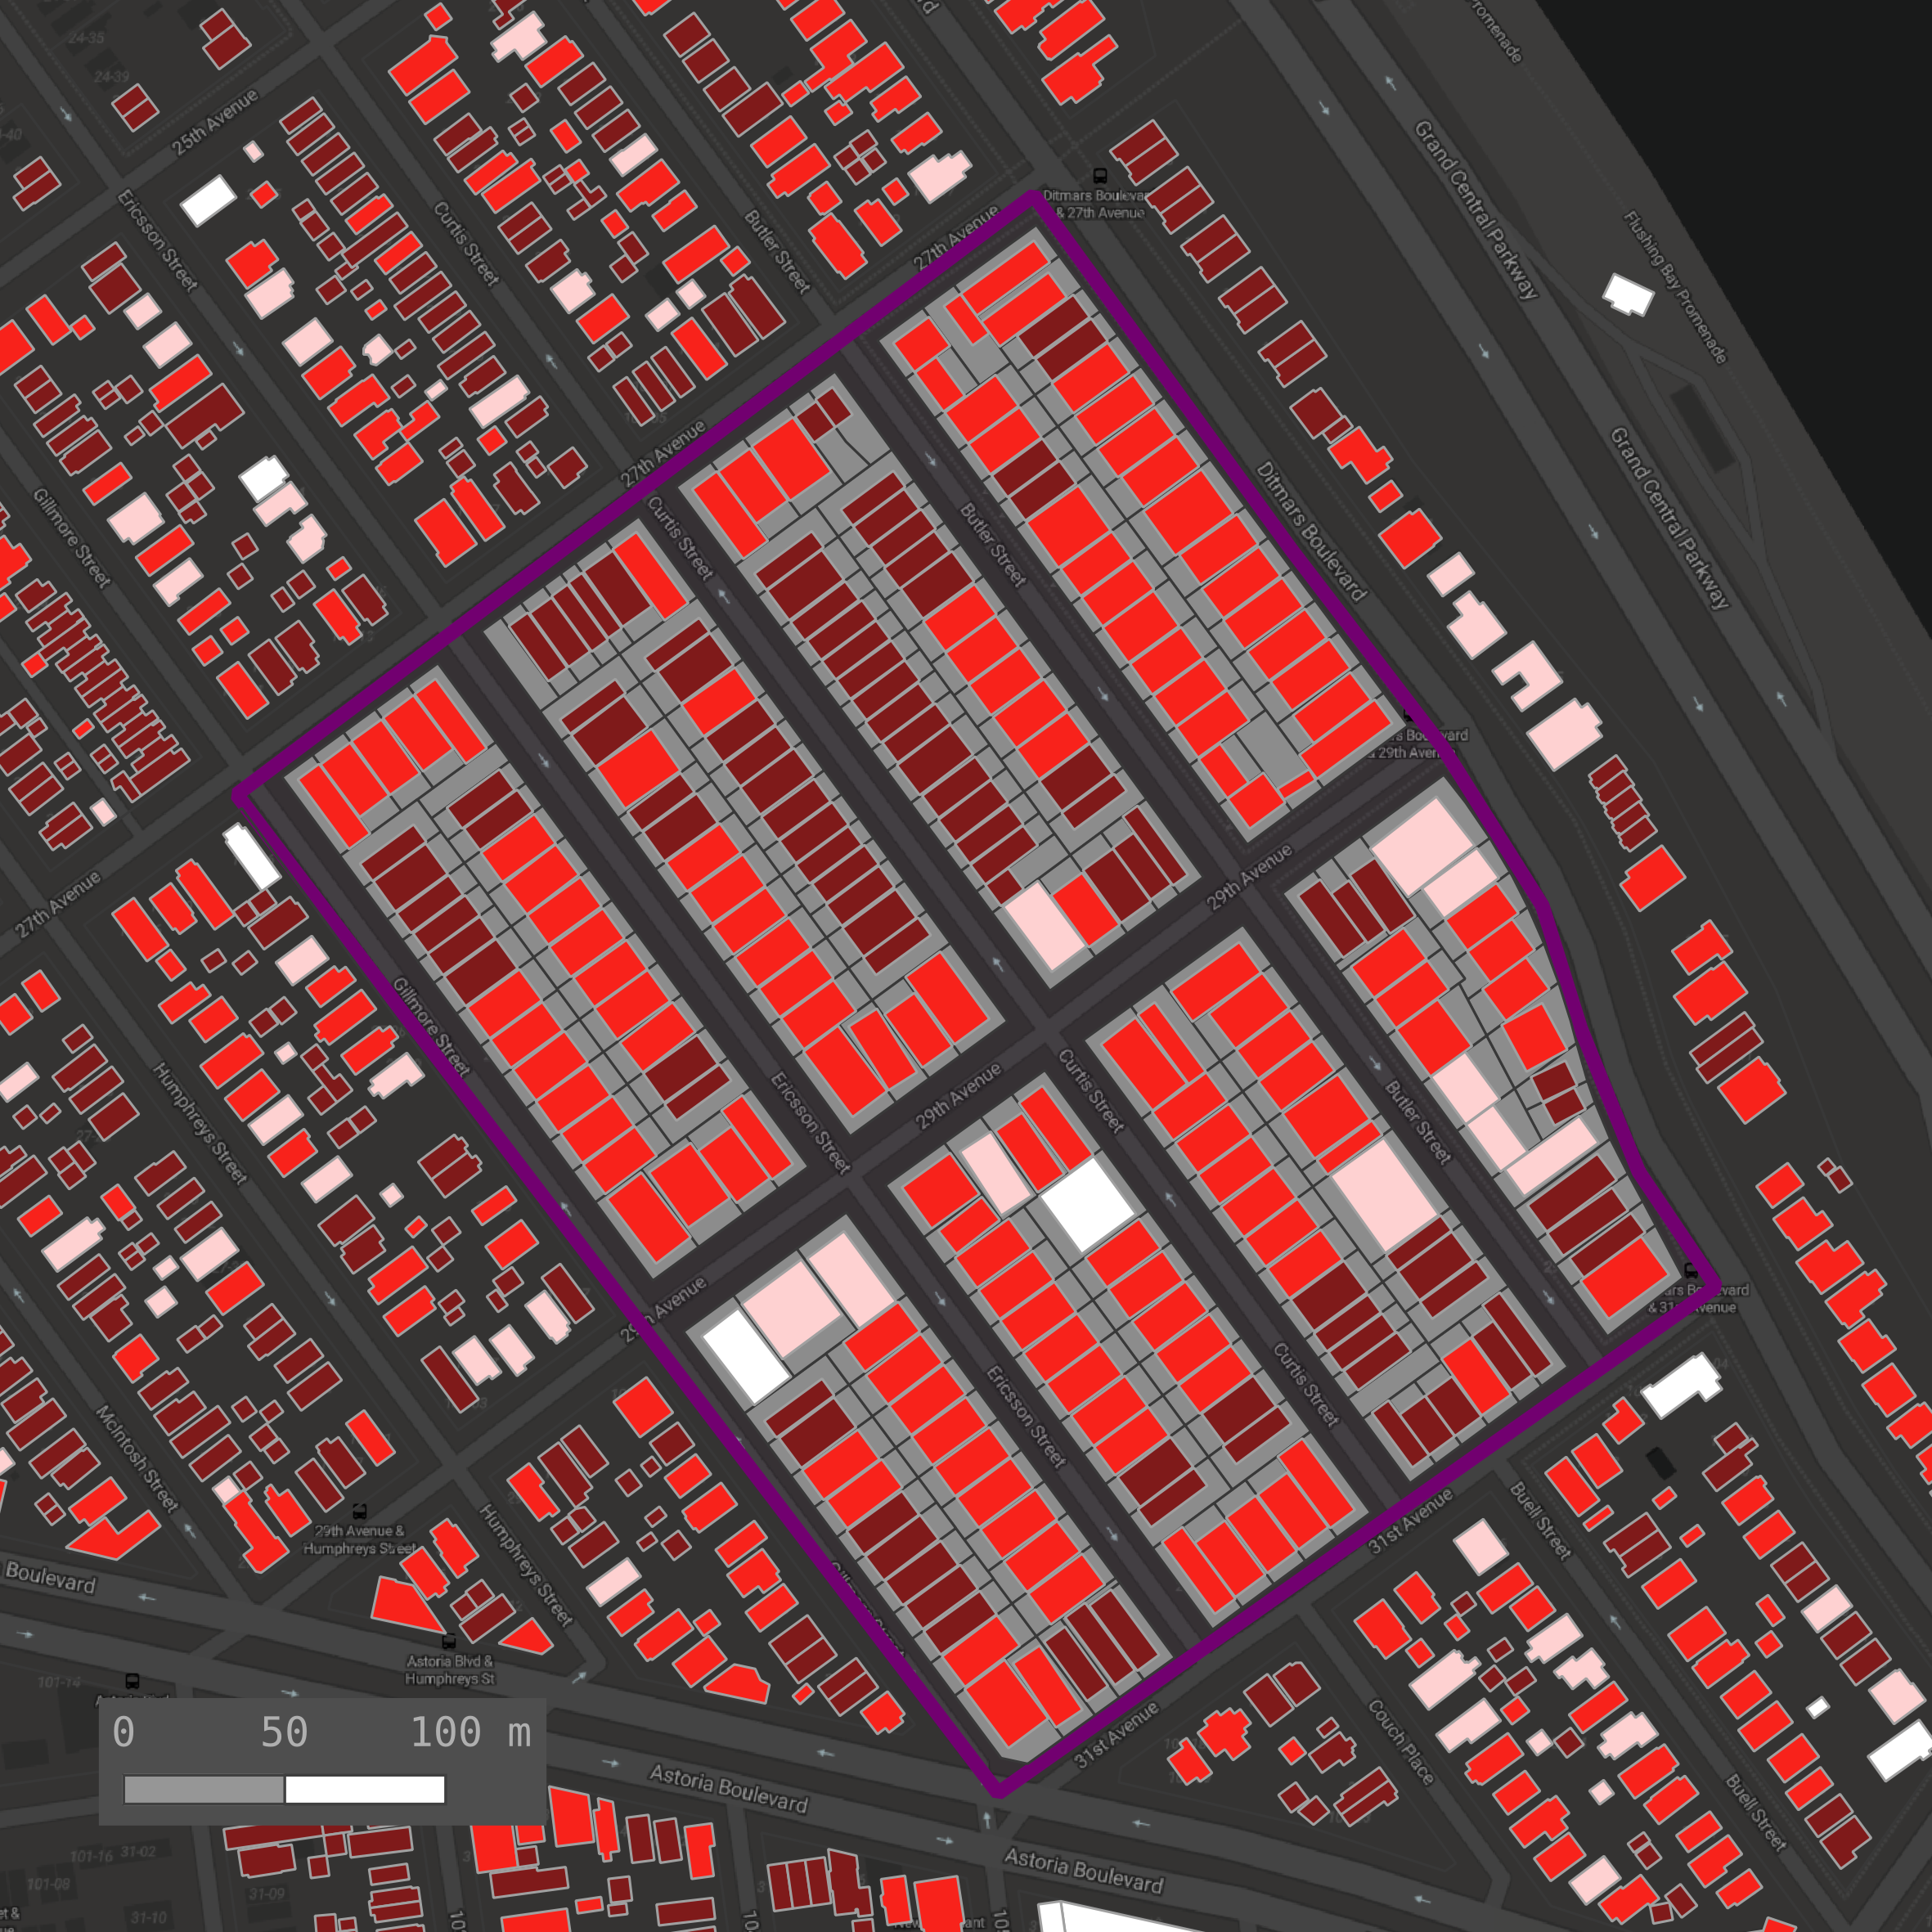
\includegraphics[width=\linewidth]{figures/buildings_6.png}	
		\end{center}
	\end{column}
	\begin{column}{0.39\linewidth}
		\justify
		\textbf{SURe project} (collaboration LASTIG, ISC-PIF, EPIDAPO)
		
		\bigskip
		
		$\rightarrow$ coupling the SimPLU3D urban generative model \cite{brasebin2017apports} with an Urban Heat Island model to find compromises between density and the UHI effect. 

	\end{column}
\end{columns}




}







\sframe{Generic multi-model of urban dynamics for SDGs trade-offs}{

\footnotesize

Other dimensions benchmarked by \cite{raimbault2020empowering} to fit population dynamics on several large urban systems


\bigskip

\textbf{Models integrated: }

\begin{itemize}
	\item Innovation diffusion urban evolution model \cite{raimbault2022trade}
	\item Marius model for economic exchanges \cite{cottineau2015modular}
	\item Co-evolution model for cities and infrastructure networks \cite{raimbault2021modeling}
\end{itemize}

\bigskip

% "semmi-weak coupling": not using workflow system - but generic

\textbf{``Semi-weak'' coupling of submodels:}

%\medskip

\begin{multline}
S_0 \rightarrow \left[ S_1^{(0)} = M_0 (S_0) \rightarrow \ldots \rightarrow S_1^{(K - 1)} = M_{K - 1} (S_1^{(K - 2)}) = S_1 \right] \longrightarrow \ldots \\
\longrightarrow \left[ S_{T}^{(0)} = M_0 (S_{T - 1}) \rightarrow \ldots \rightarrow S_T^{(K - 1)} = M_{K - 1} (S_T^{(K - 2)}) = S_T \right]
\end{multline}

\medskip

\textbf{Remarks: } strictly weak coupling does not capture dynamics nor synergies; stronger coupling may exist to better capture interdependencies processes (here no specific coupling ontology, only population and distance matrix are shared between submodels)

}


\sframe{SDGs trade-offs: optimised objectives}{

\textbf{Proxies for SDGs:}

\medskip

\begin{itemize}
	\item Total utility of innovations (SDG 9 ``Innovation'')
	\item Total spatial interaction flows across submodels (SDG 13 ``Climate'')
	\item Average distance between cities (SDG 9 ``Resilient infrastructure'')
	\item Economic inequalities (SDG 10 ``Inequalities'')
	\item Total wealth of cities (SDG 8 ``Economic Growth'')
\end{itemize}

\bigskip

\textbf{Optimisation parameters: } fixed synthetic urban system parameters but random configurations (10 repetitions); 8 parameters for innovation; 6 parameters for economic exchanges; 6 parameters for co-evolution



}


\sframe{SDGs trade-offs: optimisation results}{


\begin{center}
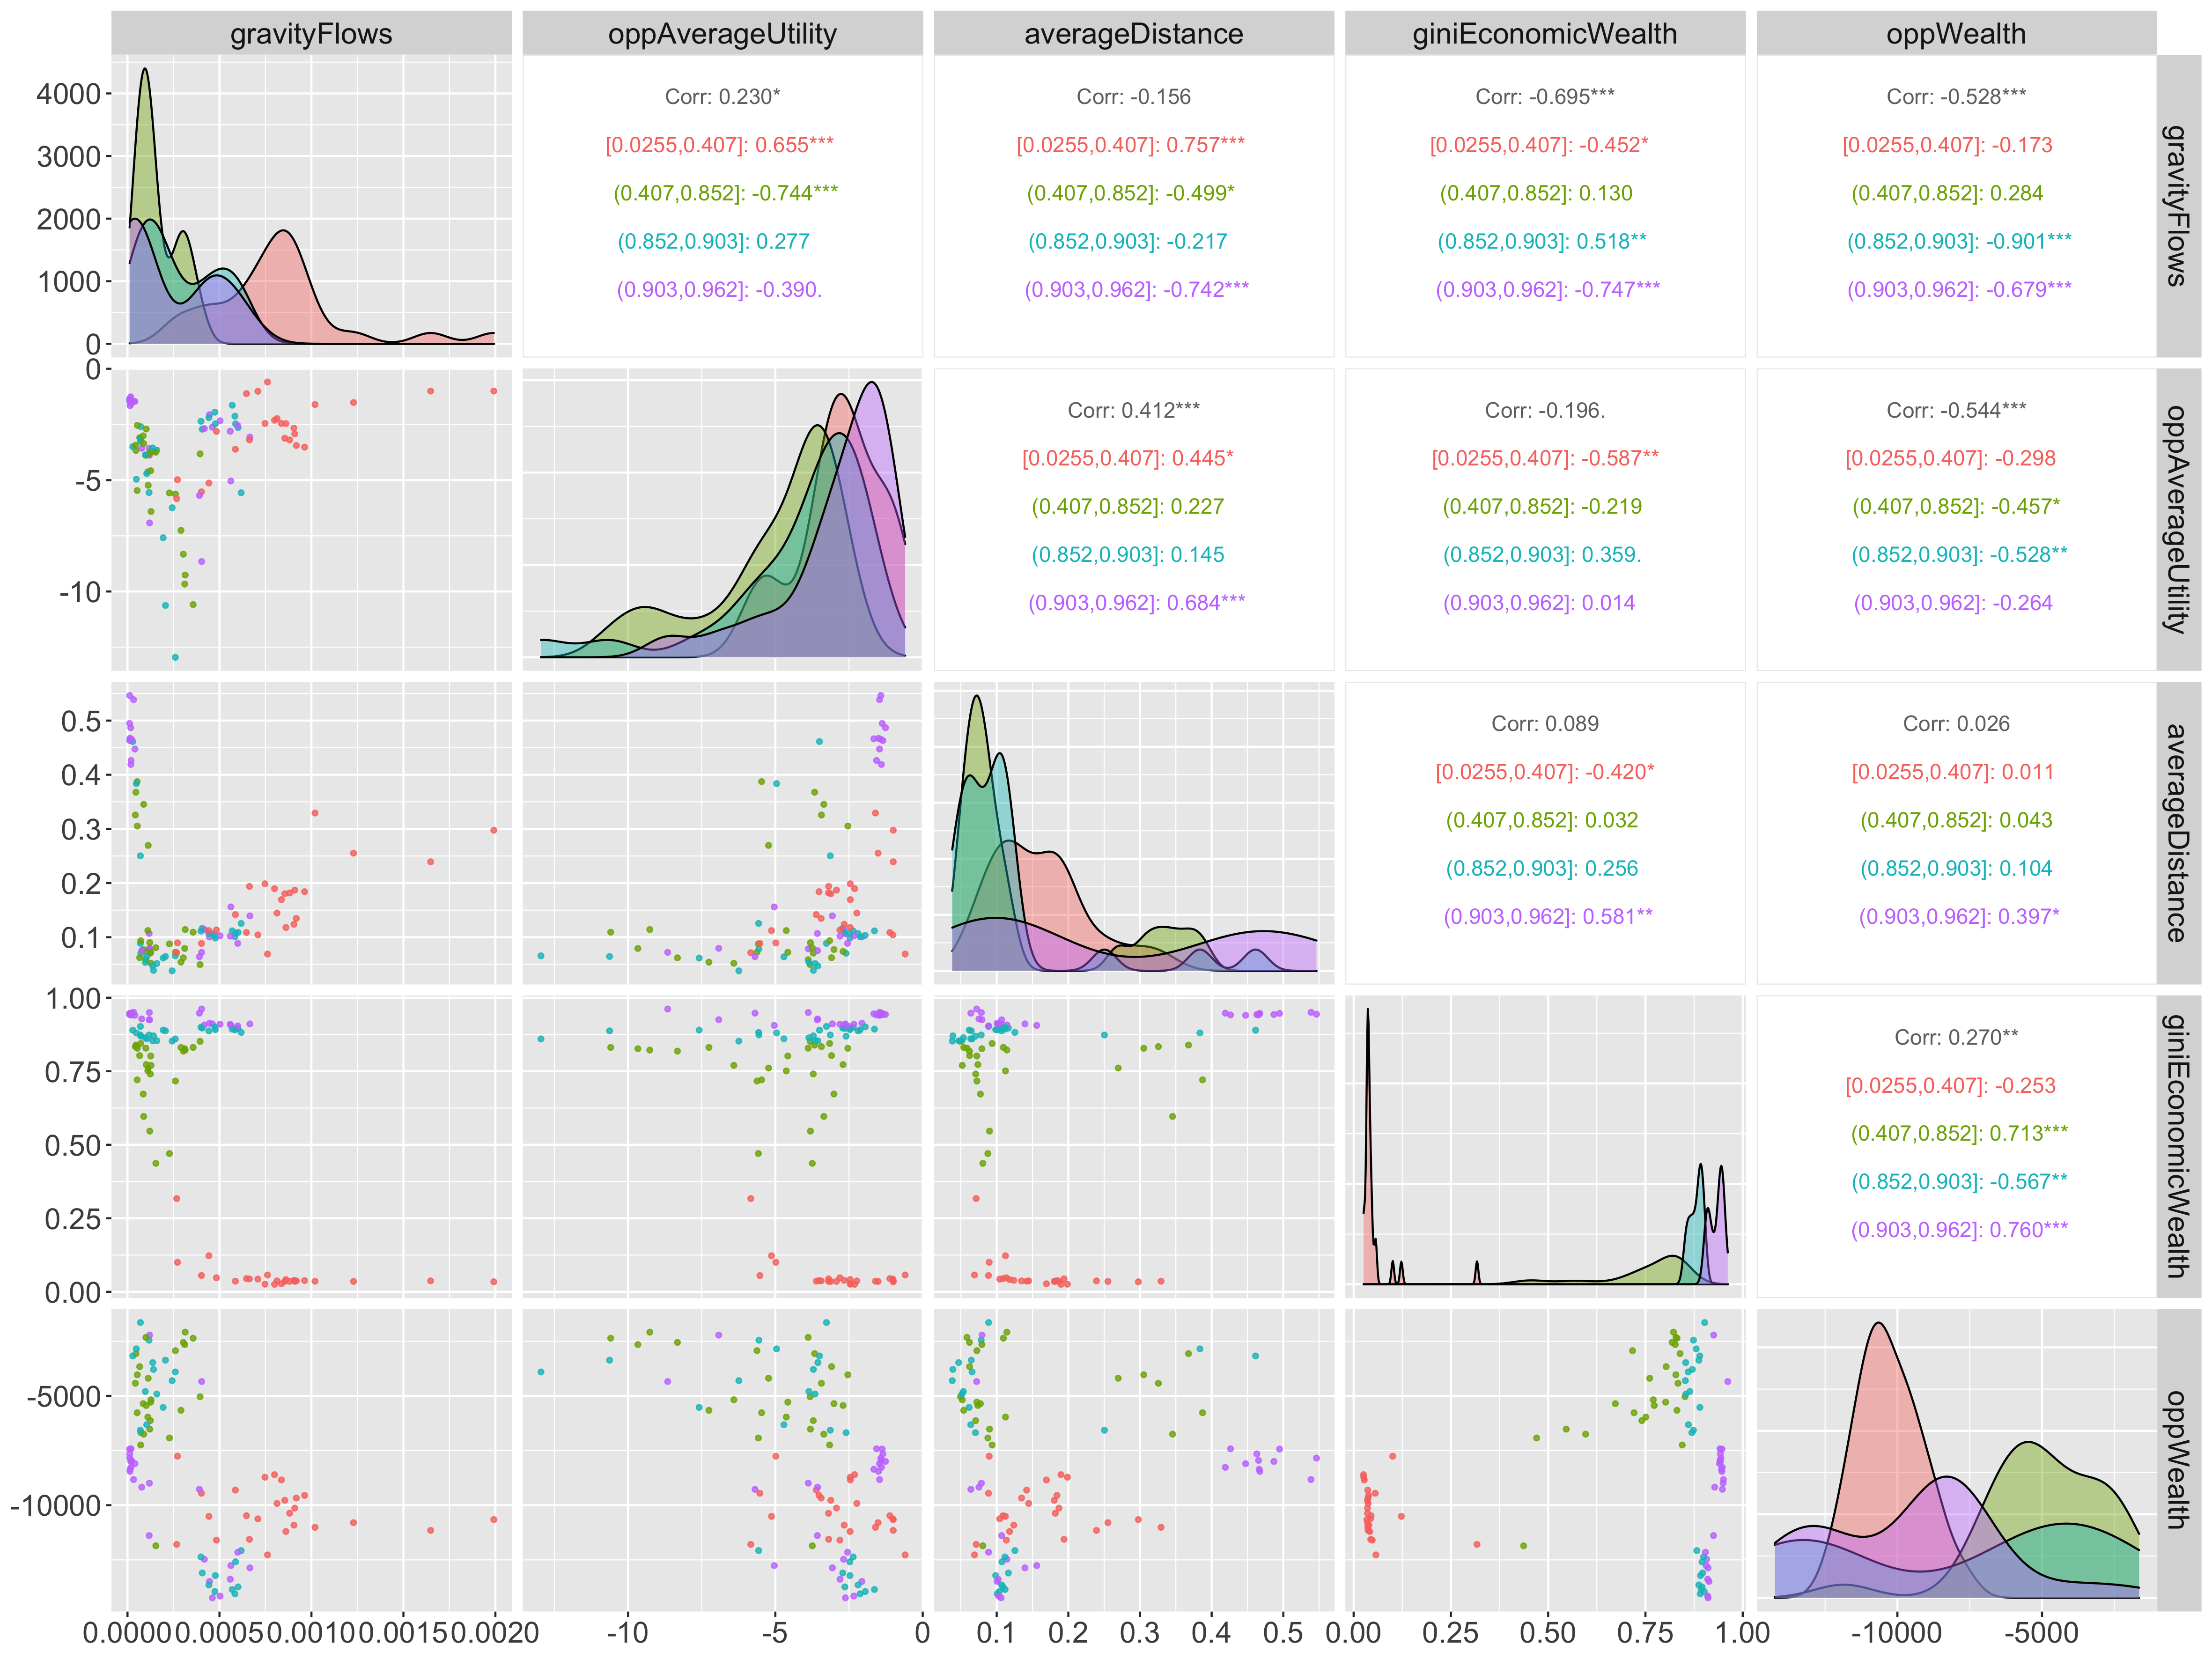
\includegraphics[width=0.86\linewidth]{figures/scatter_models_colorginiEconomicWealth_OPTIMISATION_GRID_20220622_092133.png}
\end{center}

\footnotesize
\textit{Scatterplots of the 5D Pareto front. Color level: Gini economic wealth.}

}

\sframe{SDGs trade-offs: optimisation results}{


\begin{center}
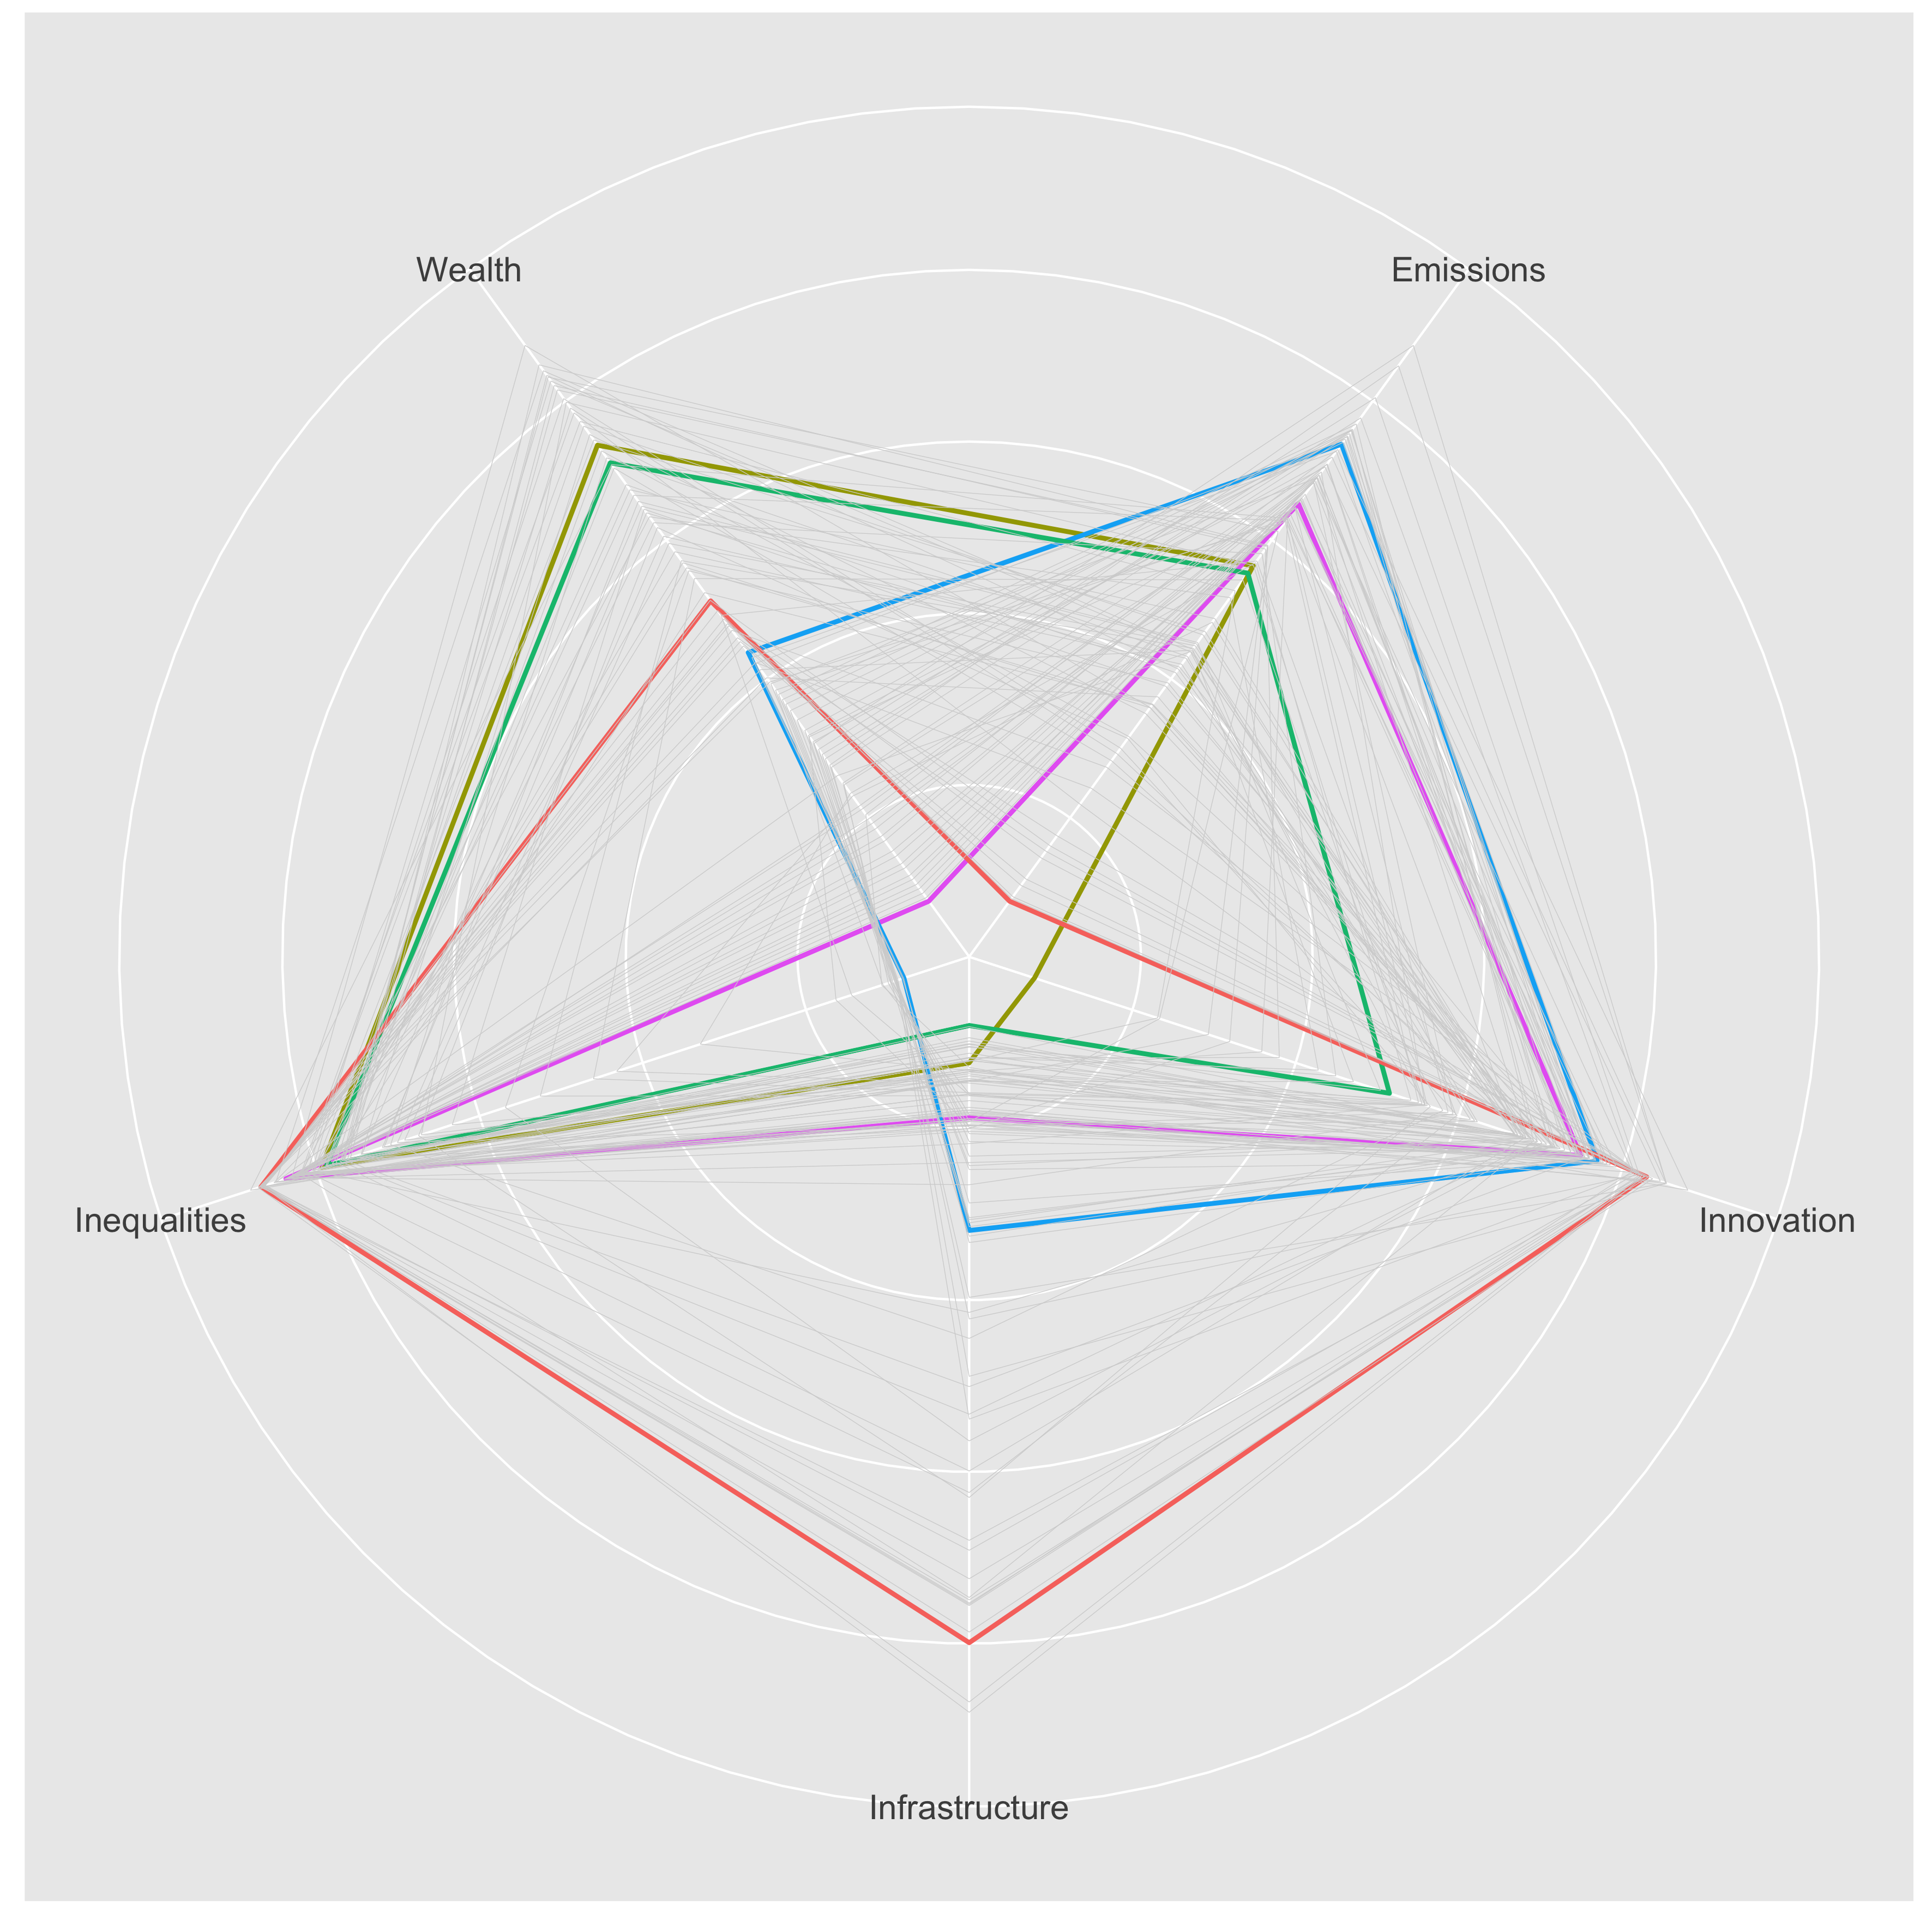
\includegraphics[width=0.65\linewidth]{figures/radar_sdgs.png}
\end{center}

\tiny
\textit{Radar plot for the many-objective optimisation (colour: best solution along each dimension)}

}



\sframe{Horizontal integration: multi-modeling and benchmarks}{


\begin{center}
	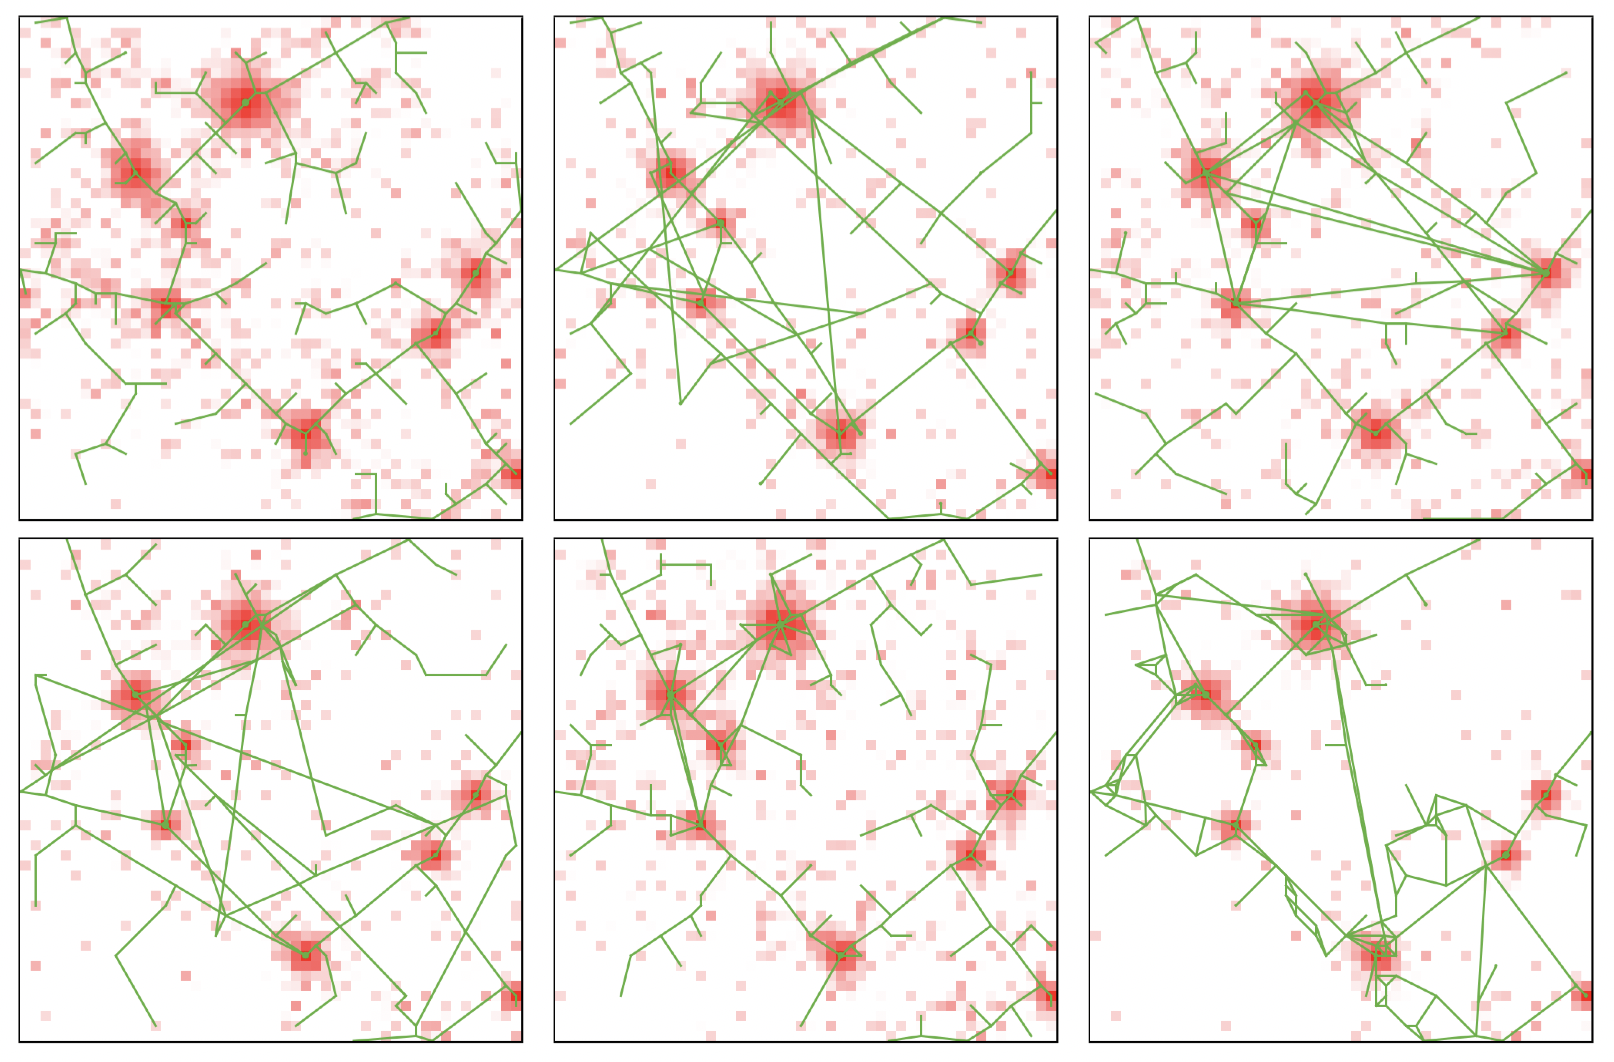
\includegraphics[width=0.56\linewidth]{figures/meso_multimodeling.png}\hspace{0.5cm}
	
\includegraphics[width=0.36\linewidth]{figures/mesobench_Fig3.png}
\end{center}

\medskip

\textit{Benchmarking network and urban morphogenesis models}


\medskip

\tiny

Raimbault, J. (2018). Multi-modeling the morphogenesis of transportation networks. In Artificial Life Conference Proceedings (pp. 382-383). MIT Press, Cambridge.

\nocite{raimbault2018multi}

\smallskip

Raimbault, J. (2020). A comparison of simple models for urban morphogenesis. arXiv preprint arXiv:2008.13277.

\nocite{raimbault2020comparison}

\smallskip

Raimbault, J. (2021). Complementarity of generative models for road networks. arXiv preprint arXiv:2109.15206.

\nocite{raimbault2021complementarity}



}




\sframe{Vertical integration: towards multi-scale models}{



\begin{center}
	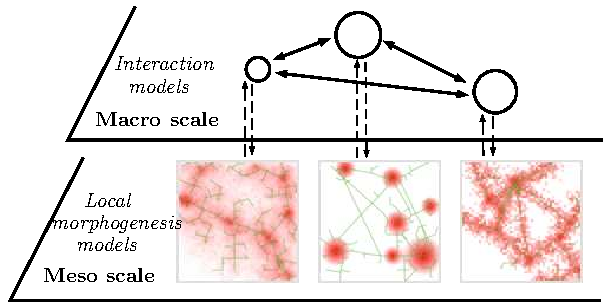
\includegraphics[width=0.75\textwidth]{figures/multiscale_morph.pdf}
\end{center}

\medskip

\textit{Processes specific to scales, coupling implies dedicated ontologies} 

\medskip

\tiny

Raimbault, J. (2021). Strong coupling between scales in a multi-scalar model of urban dynamics. arXiv preprint arXiv:2101.12725.

\nocite{raimbault2021strong}

\smallskip

Raimbault, J. (2021). A multiscale model of urban morphogenesis. arXiv preprint arXiv:2103.17241.

\nocite{raimbault2021multiscale}

\smallskip

Raimbault, J. and Pumain, D. (2023). Innovation dynamics in multi-scalar systems of cities. \textit{Under review for ALIFE 2023}.


}








\sframe{Conclusion}{

%\footnotesize

\justify

$\rightarrow$ Digital twins are a rebranding of simulation models remaining too far from human and social sciences and sustainable development goals.

\medskip

$\rightarrow$ Multiple models need to be considered, coupled and integrated, at multiple time and spatial scales, but also from multiple disciplines and approaches: \textbf{model sharing and coupling as a geo-common}.

\medskip

$\rightarrow$ These models need to be \textbf{explored, calibrated, validated}, using open tools such as OpenMOLE, in a reproducible way.

\medskip 

$\rightarrow$ All this must be \textbf{open source, shared, modular} to contribute to geo-commons and be usable for policy-making.

\medskip

$\rightarrow$ \textbf{Stakeholders} must be implied in the model development, exploration and validation process \cite{delay2020comexp}.




}




%%%%%%%%%%%%%%%%%%%%%
\begin{frame}[allowframebreaks]
\frametitle{References}
\bibliographystyle{apalike}
\bibliography{biblio}
\end{frame}
%%%%%%%%%%%%%%%%%%%%%%%%%%%%





\end{document}







